% vim: set fileencoding=UTF-8 filetype=tex :
%-----------------------------------------------------------------------------
%
% A MM1 queueing system
%
% Author: Thomas Loruenser (2013): initial version
%
%-----------------------------------------------------------------------------
% Copyright 2013, Thomas Loruenser <thomas.loruenser@ait.ac.at>
%
% This program is free software: you can redistribute it and/or modify
% it under the terms of the GNU General Public License as published by
% the Free Software Foundation, either version 3 of the License, or
% (at your option) any later version.
%
% This program is distributed in the hope that it will be useful,
% but WITHOUT ANY WARRANTY; without even the implied warranty of
% MERCHANTABILITY or FITNESS FOR A PARTICULAR PURPOSE.  See the
% GNU General Public License for more details.
%
% You should have received a copy of the GNU General Public License
% along with this program.  If not, see <http://www.gnu.org/licenses/>.
%-----------------------------------------------------------------------------
\documentclass{standalone}

\usepackage{tikz}
\usetikzlibrary{calc,arrows,positioning}

\begin{document}

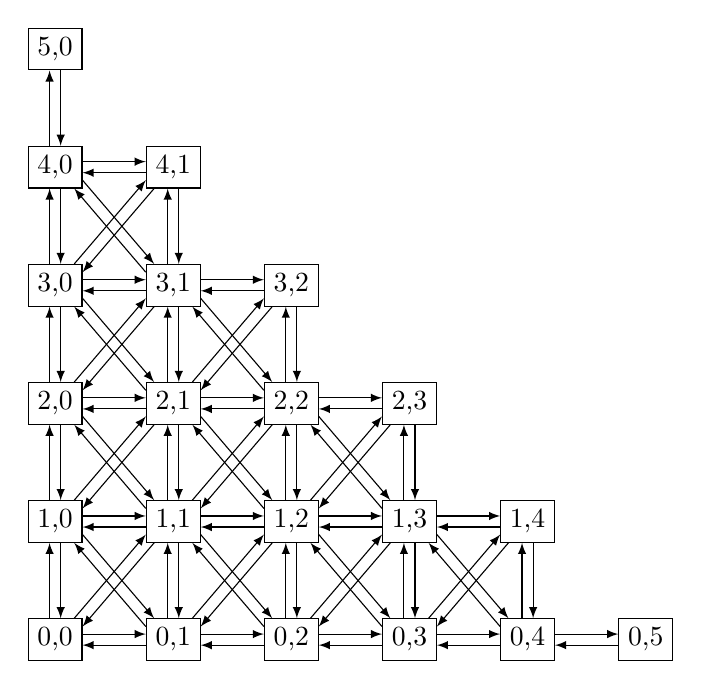
\begin{tikzpicture}
  [>=latex]
 
% important vars
\edef\size{5}

% define styles
\tikzstyle{state} = [draw, rectangle];

% define new commands
\newcommand{\conHoriz}[2]{
  \draw [->] ([yshift=0.2em] #1.east) -- ([yshift=0.2em] #2.west);
  \draw [<-] ([yshift=-0.2em] #1.east) -- ([yshift=-0.2em] #2.west);
}

\newcommand{\conVert}[2]{
  \draw [->] ([xshift=-0.2em] #1.north) to ([xshift=-0.2em] #2.south);
  \draw [<-] ([xshift=0.2em] #1.north) to ([xshift=0.2em] #2.south);
}

\newcommand{\conDiagOne}[2]{
  \draw [->] ([xshift=-0.3em] #1.north east) -- ([yshift=0.3em] #2.south west);
  \draw [<-] ([yshift=-0.3em] #1.north east) -- ([xshift=0.3em] #2.south west);
}

\newcommand{\conDiagTwo}[2]{
  \draw [->] ([yshift=0.3em] #1.south east) -- ([xshift=0.3em] #2.north west);
  \draw [<-] ([xshift=-0.3em] #1.south east) -- ([yshift=-0.3em] #2.north west);
}

% draw nodes
\foreach \y in {0,...,\size}{
  \pgfmathparse{\size-\y}
  \foreach \x in {0,...,\pgfmathresult}
    \node[state] (s\x\y) at ($1.5*(\y,\x)$) {\x,\y};
}

% draw horizontal and vertical edges
\pgfmathparse{\size-1}
\foreach \y in {0,...,\pgfmathresult}{
  \pgfmathparse{\size-1-\y}
  \foreach \x in {0,...,\pgfmathresult}{
    
    % horizontal lines s00 -- s01
    \pgfmathparse{int(\x+1)}
    \conHoriz{s\y\x}{s\y\pgfmathresult}
    
    % vertical lines from s00 -- s10
    \pgfmathparse{int(\y+1)}
    \conVert{s\y\x}{s\pgfmathresult\x}
  }
}

% draw diagonal edges
\pgfmathparse{\size-2}
\foreach \y in {0,...,\pgfmathresult}{
  \pgfmathparse{\size-2-\y}
  \foreach \x in {0,...,\pgfmathresult}{
    
    \pgfmathparse{int(\x+1)}
    \edef\xx{\pgfmathresult}
    \pgfmathparse{int(\y+1)}
    \edef\yy{\pgfmathresult}
    
    % diagonal lines from s00 -- s11
    \conDiagOne{s\y\x}{s\yy\xx}
    
    % diagonal lines from s10 -- s01
    \conDiagTwo{s\yy\x}{s\y\xx}
  }
}

\end{tikzpicture}

\end{document}

